\documentclass[xcolor=table,bigger,unknownkeysallowed]{beamer}
%\documentclass[unknownkeysallowed]{beamer}
\usepackage[utf8]{inputenc}
\usepackage[T1]{fontenc}
\usepackage[english]{babel}
\usepackage{fixltx2e}
\usepackage{graphicx}
\usepackage{epsfig}
\usepackage{longtable}
\usepackage{float}
\usepackage{wrapfig}
\usepackage{soul}
\usepackage{textcomp}
\usepackage{marvosym}
\usepackage{wasysym}
\usepackage{latexsym}
\usepackage{amssymb}
\usepackage{tabu}
\usepackage{tabularx}
\usepackage{booktabs}
\usepackage[margin=15pt,font={small,sf,it},labelfont=bf]{caption} 
\usepackage{hyperref}
\tolerance=1000
\providecommand{\alert}[1]{\textbf{#1}}
\usepackage{etoolbox}
\newcommand{\icon}[1]{\includegraphics[height=20pt,width=20pt]{#1}}
\usepackage{pgfplots}
\usepackage{tabu}
\usepackage{subcaption}
\usepackage{multirow}


\usepackage{tikz}
\usetikzlibrary{matrix,positioning,fit,fadings}
\def\drowsyColor{green!80!black}       

\title{Out of Hypervisor (OoH): Efficient Dirty Page Tracking In Userspace Using Hardware Virtualization Features}
\author{Stella Bitchebe - (bitchebe@i3s.unice.fr)\\
Advisor: Pr Alain Tchana - (alain.tchana@ens-lyon.fr) \\
ENS Lyon}
\date{~}

\usepackage{booktabs}
\usepackage[natbib=true, bibstyle=authoryear, citestyle=authoryear-comp]{biblatex}
\usepackage{beamerthemesplit}
\usetheme{progressbar}
\usecolortheme{progressbar}
\institute{\vskip1ex Rennes - April, 29}
%\subtitle{subtitle}
\definecolor{tableShade}{HTML}{787878}
\definecolor{tableShade2}{HTML}{606060}
%\setbeamersize{text margin left=.5cm,text margin right=.5cm}
\progressbaroptions{headline=none, frametitle=ckcompliant}
\newcommand{\myitem}{\item[\vspace{0.5ex}]}
\usepackage{lmodern}
\usepackage{ulem} 
\AtBeginSection[]
{
  \begin{frame}<beamer>
    %\frametitle{Outline for section \thesection}
    \tableofcontents[currentsection]
  \end{frame}
}

\setbeamersize{text margin left=0em,text margin right=0em}

\usepackage{tikz,pgfplots}
\usetikzlibrary{pgfplots.groupplots}
\usepackage{pgfplotstable}
\usepgfplotslibrary{external} 
\usetikzlibrary{patterns}
\usepgfplotslibrary{fillbetween}
\usetikzlibrary{matrix,positioning,fit,fadings}
\tikzfading[name=energyPropFading,bottom color=transparent!100,top color=transparent!0]
\usepackage{color, colortbl}
\hypersetup{}

\definecolor{codegreen}{rgb}{0,0.6,0}
\definecolor{codegray}{rgb}{0.5,0.5,0.5}
\definecolor{codepurple}{rgb}{0.58,0,0.82}
\definecolor{backcolour}{rgb}{0.95,0.95,0.92}
\definecolor{americanrose}{rgb}{1.0, 0.01, 0.24}
\definecolor{airforceblue}{rgb}{0.0, 0.0, 1.0}

\newenvironment{variableblock}[3]{%
  \setbeamercolor{block body}{#2}
  \setbeamercolor{block title}{#3}
  \begin{block}{#1}}{\end{block}}

\tikzfading[name=myfading, bottom color=transparent!100, top color=transparent!0]
\begin{document}
\thispagestyle{empty}

\maketitle

%%%%%%%%%%%%%%%%%%%%%%%%%%%%%%%%%%%%%%%%%%%%%%%%%%%%%%%%%%%%%%%%%%%%%%%%%%%%%%%%%%%
\section{Dirty Page Tracking}
%%%%%%%%%%%%%%%%%%%%%%%%%%%%%%%%%%%%%%%%%%%%%%%%%%%%%%%%%%%%%%%%%%%%%%%%%%%%%%%%%%%
        \begin{frame}
        \frametitle{Dirty Page Tracking in Userspace} 
			\begin{block}{Purpose}
				\begin{itemize}
					\item WSS (working set size) estimation
					\item Live migration
					\item Checkpointing
					\item Garbage collection
				\end{itemize}
			\end{block}		
			
			\begin{block}{Current approach}
				\begin{itemize}
					\item Page write protection
					\item Two main solutions
					\begin{itemize}
						\item Linux /proc interface
						\item Linux userfaultfd (ufd) interface
					\end{itemize}
				\end{itemize}
			\end{block}	
        \end{frame}
%%%%%%%%%%%%%%%%%%%%%%%%%%%%%%%%%%%%%%%%%%%%%%%%%%%%%%%%%%%%%%%%%%%%%%%%%%%%%%%%%%%
        \begin{frame}
			\thispagestyle{empty}
			\frametitle{Dirty Page Tracking in Userspace} 
				\begin{block}{Nomenclature}
					\begin{itemize}
						\item Tracker: the monitoring thread (e.g., CRIU, Boehm GC)
						\item Tracked: the thread whose memory is monitored (any application)
					\end{itemize}
				\end{block}		
				
				\begin{block}{Overall Functioning}
					\begin{itemize}
						\item Tracker's activity can be organized in four phases: 
						\begin{itemize}
							\item the initialization of the tracking method,
							\item the monitoring
							\item the collection of dirty page addresses
							\item the exploitation of the latter (e.g., for checkpointing)
						\end{itemize}
					\end{itemize}
				\end{block}	

				\begin{figure}
			   \centering
				   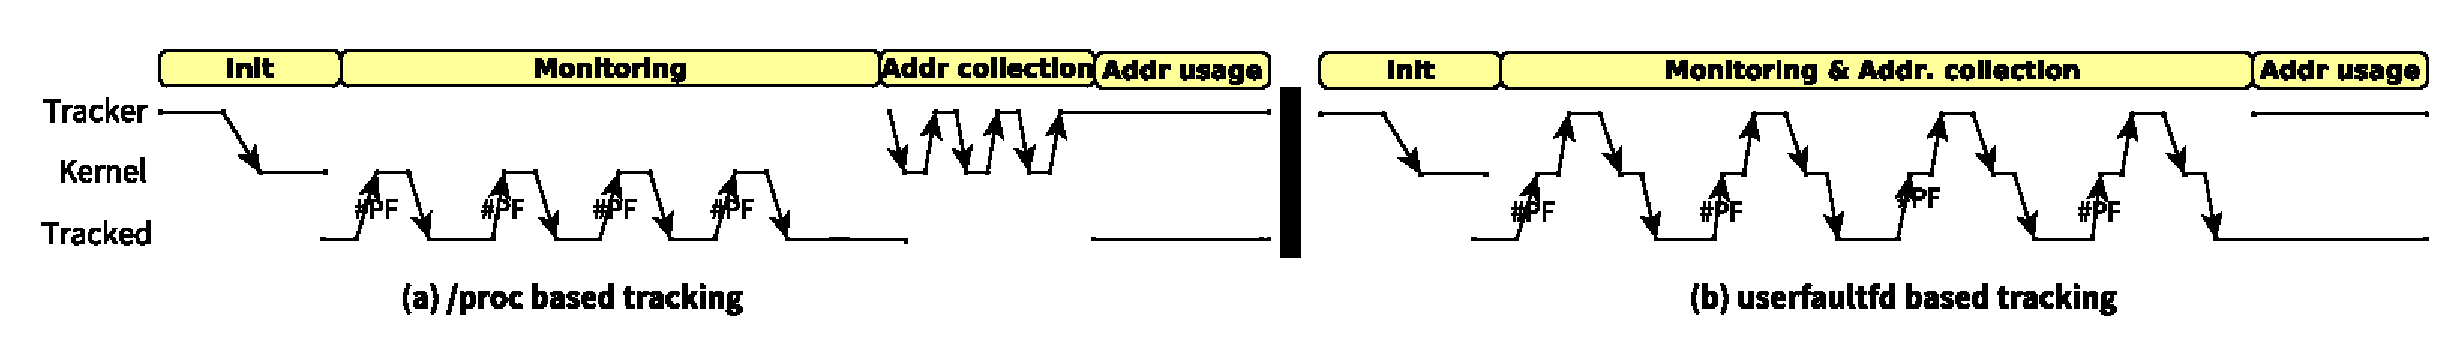
\includegraphics[width=1\columnwidth]{fig/solutions1}
			   \end{figure}
			\end{frame}
%%%%%%%%%%%%%%%%%%%%%%%%%%%%%%%%%%%%%%%%%%%%%%%%%%%%%%%%%%%%%%%%%%%%%%%%%%%%%%%%%%%
        \begin{frame}
			\frametitle{Page write protection} 
				\begin{block}{Overhead}
					\begin{itemize}
						\item ufd 
						\begin{itemize}
							\item We measured up to 15.6$\times$ and 14.5$\times$ slowdown for 1GB on Tracked and Tracker respectively
							\item Due to page fault handling and context switches
						\end{itemize}
						\item /proc 
						\begin{itemize}
							\item We measured about 2.234ms to parse the PT and flush the TLB (in the kernel), and up to 4.3$\times$ and 2.5$\times$ slowdown for 1GB on Tracked and Tracker respectively
							\item We measured about 594.187ms to parse the PT in userspace (/proc/PID/pagemap) for 1GB				
						\end{itemize}					
					\end{itemize}
				\end{block}				
			\end{frame}                   
	%%%%%%%%%%%%%%%%%%%%%%%%%%%%%%%%%%%%%%%%%%%%%%%%%%%%%%%%%%%%%%%%%%%%%%%%%%%%%%%%%%%   
\section{OoH for PML}
%%%%%%%%%%%%%%%%%%%%%%%%%%%%%%%%%%%%%%%%%%%%%%%%%%%%%%%%%%%%%%%%%%%%%%%%%%%%%%%%%%%
        \begin{frame}
		\thispagestyle{empty}
        \frametitle{Intel PML} 
			\begin{block}{Functioning}
 		    \begin{figure}
				\centering
				\fcolorbox{white}{white}{					
				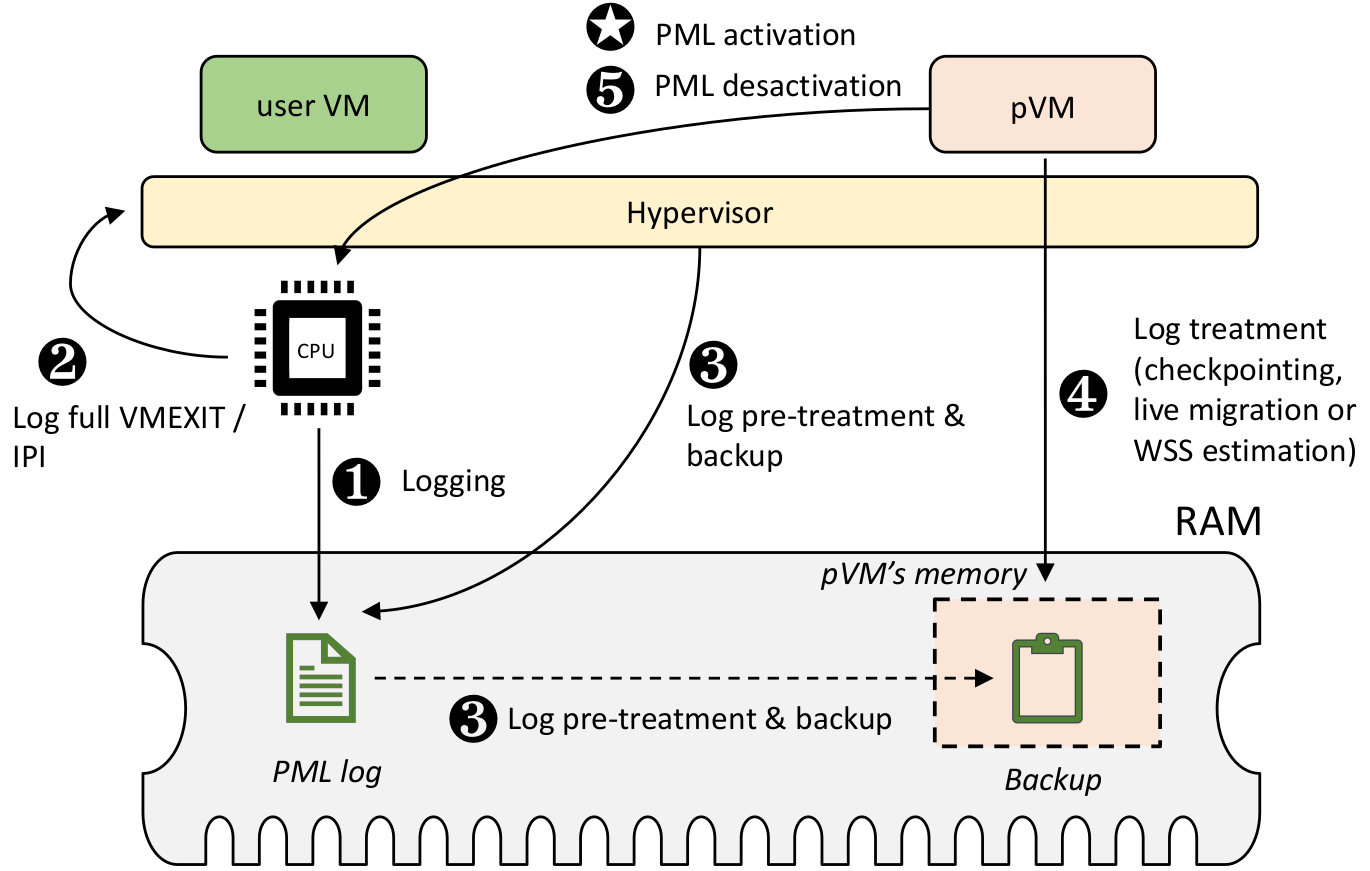
\includegraphics[width=.55\columnwidth]{fig/pml_actual}
				}
			\end{figure}
			\end{block}
			\begin{block}{Intel PML in the OoH Context}
				\begin{itemize}
					\item To accelerate CRIU checkpointing and Boehm garbage collection
				\end{itemize}
			\end{block}				
        \end{frame}
%%%%%%%%%%%%%%%%%%%%%%%%%%%%%%%%%%%%%%%%%%%%%%%%%%%%%%%%%%%%%%%%%%%%%%%%%%%%%%%%%%%
        \begin{frame}
        \frametitle{Dirty page tracking in userspace (with PML)} 
 		    \begin{figure}
			\centering
				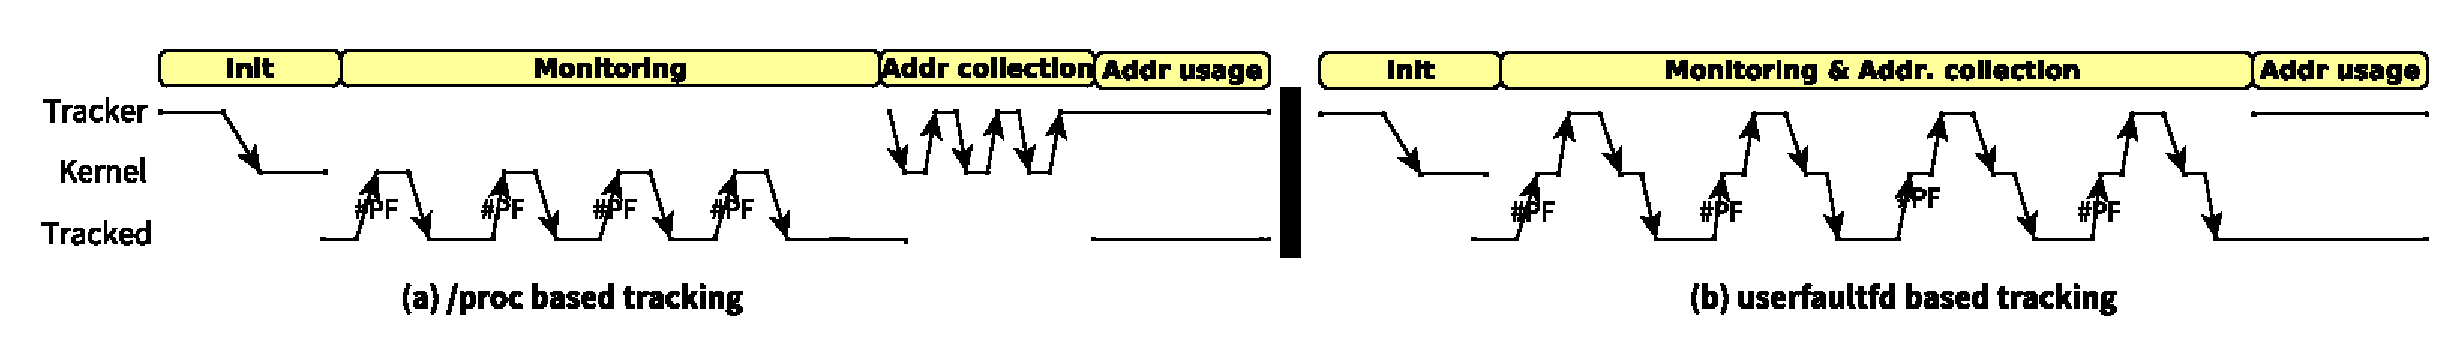
\includegraphics[width=1\columnwidth]{fig/solutions1}
			\end{figure}
~\\			
~\\
 		    \begin{figure}
			\centering
				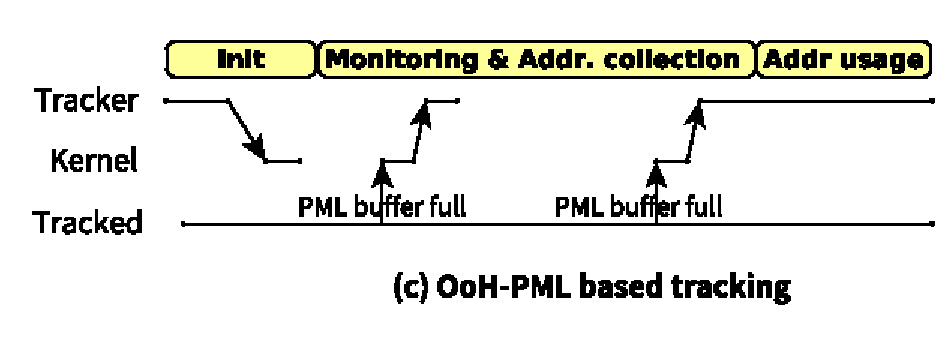
\includegraphics[width=.5\columnwidth]{fig/solutions2}				
			\end{figure}							
        \end{frame}          
%%%%%%%%%%%%%%%%%%%%%%%%%%%%%%%%%%%%%%%%%%%%%%%%%%%%%%%%%%%%%%%%%%%%%%%%%%%%%%%%%%%
        \begin{frame}
                \frametitle{OoH for PML}			
			\begin{block}{Challenges}
				\begin{itemize}
					\item ($C_1$) PML can only be managed by the hypervisor
					\item ($C_2$) PML works at coarse-grained, that is it concerns the entire VM
					\item ($C_3$) PML only logs GPAs
				\end{itemize}
			\end{block} 
        \end{frame}         
%%%%%%%%%%%%%%%%%%%%%%%%%%%%%%%%%%%%%%%%%%%%%%%%%%%%%%%%%%%%%%%%%%%%%%%%%%%%%%%%%%%
        \begin{frame}
            \frametitle{OoH for PML}			
			\begin{block}{Two Solutions}
				\begin{itemize}
					\item Extended PML (EPML): small hardware changes
					\item Shadow PML (SPML): no hardware modification					
					\begin{itemize}
						\item Its huge overhead justifies EPML
					\end{itemize}
				\end{itemize}
			\end{block} 
        \end{frame}  
%%%%%%%%%%%%%%%%%%%%%%%%%%%%%%%%%%%%%%%%%%%%%%%%%%%%%%%%%%%%%%%%%%%%%%%%%%%%%%%%%%%
        \begin{frame}
			\thispagestyle{empty}
			\frametitle{OoH for PML}			
			\begin{block}{SPML Design}
				\begin{figure}
				\centering
				\fcolorbox{white}{black}{	                					
					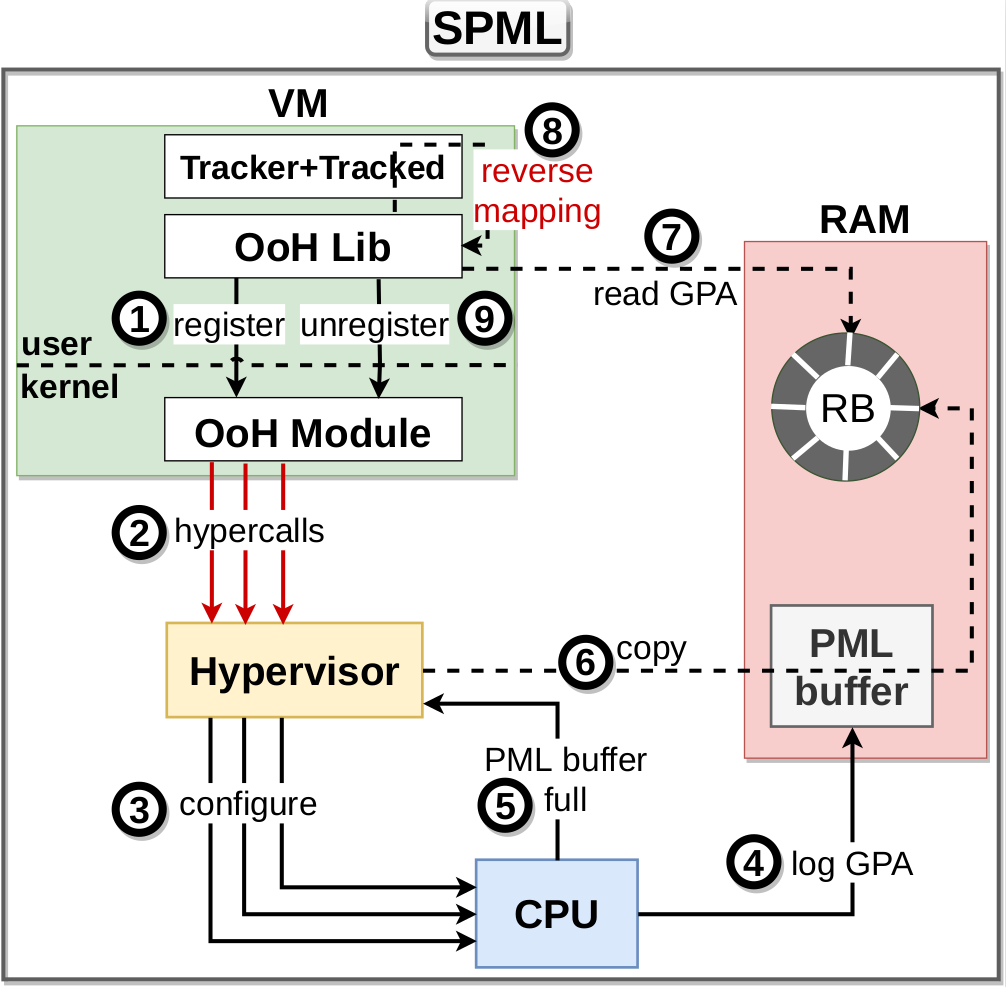
\includegraphics[width=.5\linewidth]{fig/spml.png}
				}				
				\end{figure}
			\end{block}		
        \end{frame}
%%%%%%%%%%%%%%%%%%%%%%%%%%%%%%%%%%%%%%%%%%%%%%%%%%%%%%%%%%%%%%%%%%%%%%%%%%%%%%%%%%%
        \begin{frame}
			\thispagestyle{empty}
			\frametitle{OoH for PML}
			\begin{block}{SPML limitations}
				\begin{overprint}

				\onslide<1>
				\begin{itemize}
					\item Costly reverse mapping (takes about $15.739 \: s$ for 1GB working set)
					\begin{figure}[!h]
						\fcolorbox{white}{white}{	
						\centering 
						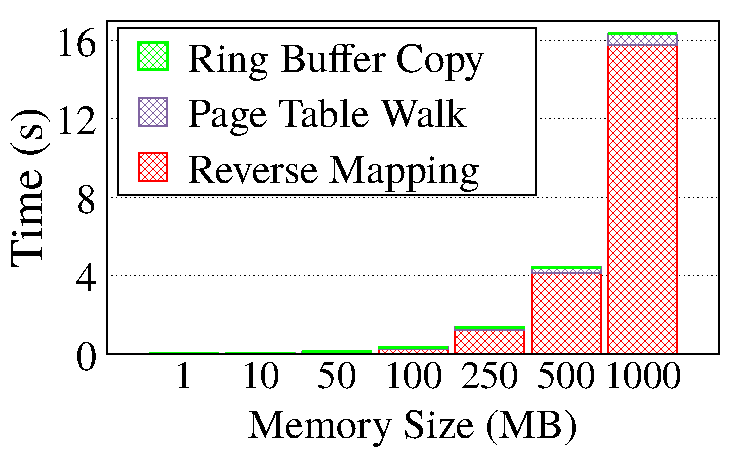
\includegraphics[width=.55\linewidth]{fig/bottleneck}%
						}		
						\captionof{figure}{\small Reverse mapping appears to be the bottleneck of SPML.}
						\label{fig:spml-bottleneck}
					\end{figure}
				\end{itemize}

				\onslide<2>
				\begin{itemize}
					\item Costly reverse mapping (takes about $15.739 \: s$ for 1GB working set)
					\item Costly hypercalls ($4.49 \mu s$ to perform an empty hypercall)
				\end{itemize}

			\end{overprint}

			\end{block} 
        \end{frame}
%%%%%%%%%%%%%%%%%%%%%%%%%%%%%%%%%%%%%%%%%%%%%%%%%%%%%%%%%%%%%%%%%%%%%%%%%%%%%%%%%%%
        \begin{frame}
			\thispagestyle{empty}
			\frametitle{OoH for PML}			
			\begin{block}{EPML Design}
				\begin{figure}
				\centering
				\fcolorbox{white}{black}{	                					
					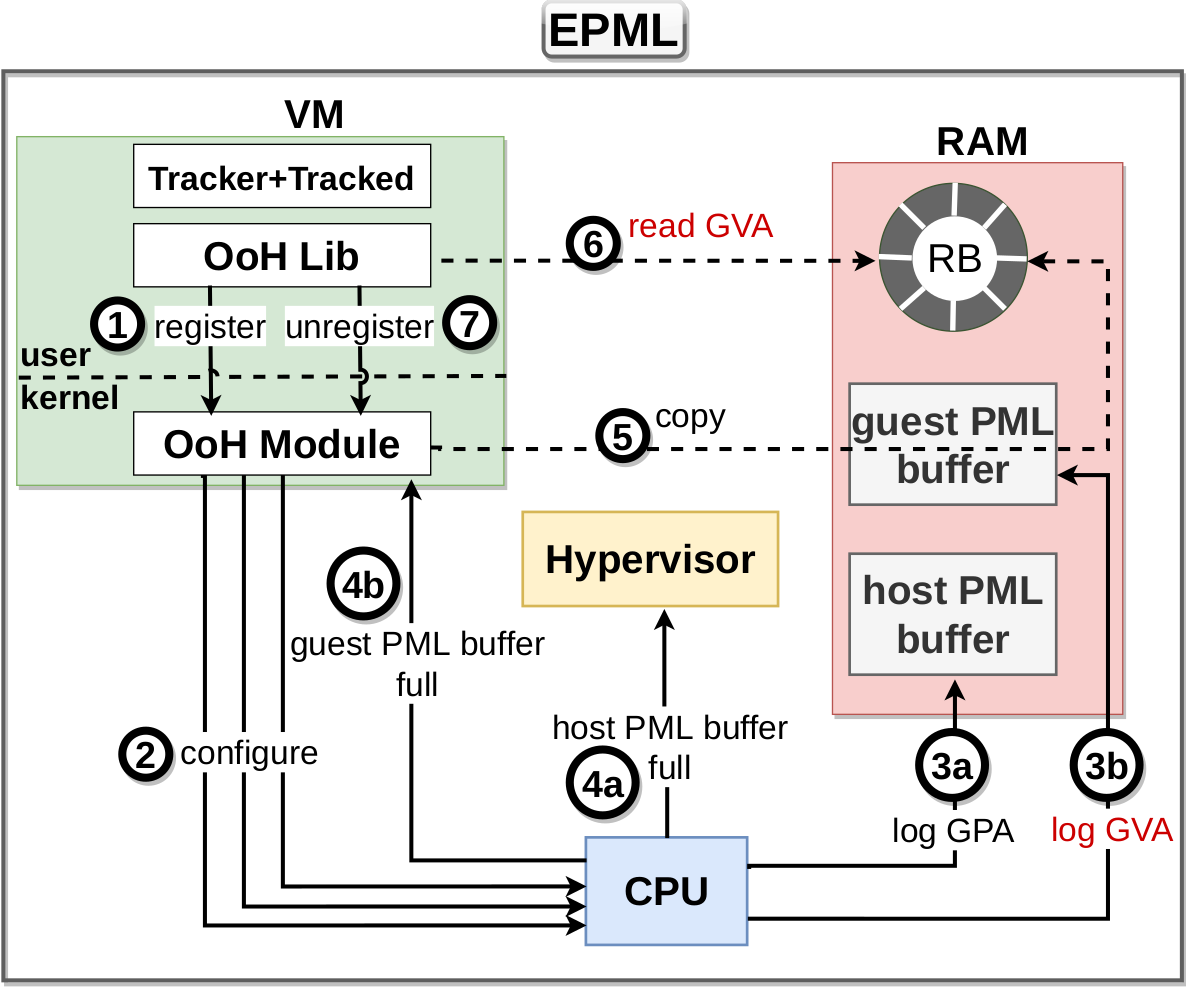
\includegraphics[width=.5\columnwidth]{fig/epml.png}
				}				
				\end{figure}
			\end{block}		
        \end{frame}
%%%%%%%%%%%%%%%%%%%%%%%%%%%%%%%%%%%%%%%%%%%%%%%%%%%%%%%%%%%%%%%%%%%%%%%%%%%%%%%%%%%
        \begin{frame}
            \frametitle{OoH for PML}			
			\begin{block}{EPML}
				\begin{itemize}
					\item We leverage VMCS shadowing to allow the guest to perform \texttt{vmread} and \texttt{vmwrite} instructions
					\item At load time, OoH Module calls the hypervisor to enable and configure VMCS shadowing
				\end{itemize}
			\end{block} 
        \end{frame} 
%%%%%%%%%%%%%%%%%%%%%%%%%%%%%%%%%%%%%%%%%%%%%%%%%%%%%%%%%%%%%%%%%%%%%%%%%%%%%%%%%%%
        \begin{frame}
                \frametitle{OoH for PML}			
			\begin{block}{Hardware changes}
				\begin{itemize}
					\item We introduce in VMCS's VM-Execution Control area a new field (called \texttt{Guest PML Address})
					\item We extend the PT walk to make the processor log GVA to the guest-level PML buffer and the GPA to the hypervisor-level PML buffer.
					\item We modify the hardware so that when the guest-level PML buffer is full, the processor raises a virtual self-IPI (Inter-Processor Interrupt)
				\end{itemize}
			\end{block} 
        \end{frame}     
%%%%%%%%%%%%%%%%%%%%%%%%%%%%%%%%%%%%%%%%%%%%%%%%%%%%%%%%%%%%%%%%%%%%%%%%%%%%%%%%%%%
        \begin{frame}
            \frametitle{OoH for PML}			
			\begin{block}{Implementation}
				\begin{itemize}
					\item We implemented EPML's hardware changes in BOCHS				
					\item We used Xen as the hypervisor and Linux as the guest OS
					\item We integrated OoH Lib with CRIU and Boehm GC
				\end{itemize}
			\end{block} 
        \end{frame}
%%%%%%%%%%%%%%%%%%%%%%%%%%%%%%%%%%%%%%%%%%%%%%%%%%%%%%%%%%%%%%%%%%%%%%%%%%%%%%%%%%%
        \begin{frame}
                \frametitle{OoH for PML}			
			\begin{block}{Benchmarks}
				\begin{itemize}
					\item Macro-benchmarks: tkrzw~\cite{tkrzw} applications (key value store) and Phoenix applications (MapReduce)
					\item We considered three working set sizes (Small, Medium and Large)
				\end{itemize}
			\end{block} 			
        \end{frame}  
%%%%%%%%%%%%%%%%%%%%%%%%%%%%%%%%%%%%%%%%%%%%%%%%%%%%%%%%%%%%%%%%%%%%%%%%%%%%%%%%%%%
        \begin{frame}
            \frametitle{OoH for PML}			
			\begin{block}{Evaluations}
				\begin{itemize}
					\item What is the potential overhead or improvement of SPML and EPML compared to \texttt{/proc} and \texttt{ufd}?
					\item What is the scalability of SPML and EPML?
					\item How to accurately evaluate EPML?
					\item Approach
					\begin{itemize}
						\item build a formula
						\item show the accuracy of that formula on other techniques, which are measurable
						\item by construction, the formula is accurate for EPML
					\end{itemize}
				\end{itemize}
			\end{block} 
        \end{frame} 
%%%%%%%%%%%%%%%%%%%%%%%%%%%%%%%%%%%%%%%%%%%%%%%%%%%%%%%%%%%%%%%%%%%%%%%%%%%%%%%%%%%
        \begin{frame}
                \frametitle{Evaluations}			
			\begin{block}{Formulas: Impact on Tracker}
				\begin{itemize}
					\item The execution time of Tracker when it implements technique $x$
					\begin{equation}
						E(C_{tker}) = E(C_{x}) + E(C_{p}) + I(C_{x},C_{p})
						\label{eq:formula-generic}
					\end{equation}
					where $E(C)$ is the execution time of code $C$ and $I(C_1,C_2)$ is the impact of $C_1$ on $C_2$.
				\end{itemize}
			\end{block} 
        \end{frame}                                                                              
%%%%%%%%%%%%%%%%%%%%%%%%%%%%%%%%%%%%%%%%%%%%%%%%%%%%%%%%%%%%%%%%%%%%%%%%%%%%%%%%%%%  
        \begin{frame}
			\frametitle{Evaluations}
			\begin{block}{Formulas: Impact on Tracker}
				\begin{equation}\scriptsize
					\begin{split}
						E(C_{/proc}) = & \; E(C_{echo \; 4 \; > \; /proc/PID/clear\_refs}) \\
									& + E(C_{page \; table \; walk \; in \; userspace}) \\
						E(C_{UFD}) = & \; E(C_{ioctl \; write\_protect}) \\
									& + E(C_{ioctl \; register}) \\
									& + E(C_{ioctl \; write\_unprotect}) \\
						E(C_{SPML}) = & \; E(C_{ring \; buffer \; copy}) \\
									& + E(C_{reverse \; mapping}) \\
									& + E(C_{enable/disable \; PML}) \\
						E(C_{EPML}) = & \; E(C_{ring \; buffer \; copy}) \\
									& + E(C_{enable/disable \; PML})
					\end{split}
					\label{eq:formula-detailed}
				\end{equation}								
			\end{block}
        \end{frame}
%%%%%%%%%%%%%%%%%%%%%%%%%%%%%%%%%%%%%%%%%%%%%%%%%%%%%%%%%%%%%%%%%%%%%%%%%%%%%%%%%%%
        \begin{frame}
            \frametitle{Evaluations}			
			\begin{block}{Formulas: Impact on Tracked}
				\begin{itemize}
					\item The execution time of Tracked when it is monitored by a tracker using the technique $x$:
					\begin{equation}
						\small
						\label{eq:formula-tracked}
						E(C_{tked\_tker}) = E(C_{tked}) + E(C_{tker}) + I(C_{x},C_{tked})
					\end{equation}
					where $I(C_{x},C_{tked})$ consists of page faults, vmexits, etc..
					Thus, the overhead of $x$ on Tracked is $E(C_{tker}) + I(C_{x},C_{tked})$. 
				\end{itemize}
			\end{block} 
        \end{frame}        
%%%%%%%%%%%%%%%%%%%%%%%%%%%%%%%%%%%%%%%%%%%%%%%%%%%%%%%%%%%%%%%%%%%%%%%%%%%%%%%%%%%
        \begin{frame}
			\frametitle{Evaluations}
			\begin{block}{Formulas: Impact on Tracked}
				\begin{equation}\scriptsize
					\begin{split}
						I(C_{/proc},C_{tked}) = & \; E(C_{PFH \; in \; kernelspace})\\
												& + E(C_{context \; switch})\\
						I(C_{UFD},C_{tked}) = & \; E(C_{PFH \; in \; userspace})\\
											& + E(C_{context \; switch}) \\
						I(C_{SPML},C_{tked}) = & \; E(C_{vmexits}) \\
											& + N \times E(C_{vmread/vmwrite})\\
						I(C_{EPML},C_{tked}) = & \; N \times E(C_{vmread/vmwrite})	
					\end{split}
					\label{eq:formula-impact-detailed}
				\end{equation}		
				For $I(C_{EPML},C_{tked})$, we use SPML's N (the number of context switches) as it is the same (validated by running SPML and EPML under BOCHS).
			\end{block}
        \end{frame}   
%%%%%%%%%%%%%%%%%%%%%%%%%%%%%%%%%%%%%%%%%%%%%%%%%%%%%%%%%%%%%%%%%%%%%%%%%%%%%%%%%%%  
        \begin{frame}
            \frametitle{Formulas: Validation}
			\begin{table}[h]
				\centering \scriptsize
				\begin{subtable}[b]{.45\textwidth}
					\centering 
					\begin{tabular}{l l}
						\toprule
						\hline
						Metric & Time (ms) \\
						\hline
						\textcolor{americanrose}{\textbf{$E(C_{tker})$}} & \\
						\textcolor{americanrose}{\textbf{measured}} & \multirow{-2}{*}{\textcolor{americanrose}{\textbf{5503.79}}}\\
						\textcolor{airforceblue}{\textbf{$E(C_{tked\_tker})$}} & \\
						\textcolor{airforceblue}{\textbf{measured}} & \multirow{-2}{*}{\textcolor{airforceblue}{\textbf{135255.35}}}\\
						\midrule
						$E(C_{p})$ & 251.35\\
						$E(C_{copy\_rb})$ & 0.49\\
						$E(C_{disable \; pml})$ & 2.06\\
						$E(C_{rev. \; mapping})$ & 5419 \\
						\textcolor{americanrose}{\textbf{$E(C_{tker})$}}  &\\
						\textcolor{americanrose}{\textbf{estimated}} &  \multirow{-2}{*}{\textcolor{americanrose}{\textbf{5672.9}}}\\
						\midrule
						$E(C_{vmexits})$ & 18000\\
						$N$ & 39\\
						$E(C_{vmread,vmwrite})$ & $1.73 \times 10^{-3}$\\
						\textcolor{airforceblue}{\textbf{$E(C_{tked\_tker})$}}  & \\
						\textcolor{airforceblue}{\textbf{estimated}} & \multirow{-2}{*}{\textcolor{airforceblue}{\textbf{136919.85}}}\\
						\bottomrule
					\end{tabular}
					\subcaption{SPML}
					\label{tab:criu-spml-formula}
				\end{subtable}
				\hfill
				\begin{subtable}[b]{.45\textwidth}
					\centering 
					\begin{tabular}{l l}
						\toprule
						\hline
						Metric & Time (ms) \\
						\hline
						\textcolor{americanrose}{\textbf{$E(C_{tker})$}} & \\
						\textcolor{americanrose}{\textbf{measured}} & \multirow{-2}{*}{\textcolor{americanrose}{\textbf{1097.99}}}\\
						\textcolor{airforceblue}{\textbf{$E(C_{tked\_tker})$}} & \\
						\textcolor{airforceblue}{\textbf{measured}} & \multirow{-2}{*}{\textcolor{airforceblue}{\textbf{115283.98}}}\\
						\midrule
						$E(C_{p})$ & 251.35\\
						$E(C_{clear\_refs})$ & 1.409\\
						$E(C_{PT walk})$ & 0.89\\
						\textcolor{americanrose}{\textbf{$E(C_{tker})$}}  & \\
						\textcolor{americanrose}{\textbf{estimated}} & \multirow{-2}{*}{\textcolor{americanrose}{\textbf{1116.09}}}\\
						\midrule
						$E(C_{PFH user})$ & 0.27\\
						\textcolor{airforceblue}{\textbf{$E(C_{tked\_tker})$}}  &\\
						\textcolor{airforceblue}{\textbf{estimated}} &  \multirow{-2}{*}{\textcolor{airforceblue}{\textbf{114418.58}}}\\
						\bottomrule
					\end{tabular}
					\subcaption{\texttt{/proc}}
					\label{tab:criu-proc-formula}
				\end{subtable}
				\vspace{.3cm}
				\caption{An accuracy of 96.34\% and 99\% respectively}
				\vspace{.3cm}
			\end{table}
        \end{frame}  
%%%%%%%%%%%%%%%%%%%%%%%%%%%%%%%%%%%%%%%%%%%%%%%%%%%%%%%%%%%%%%%%%%%%%%%%%%%%%%%%%%%
        \begin{frame}
			\frametitle{Evaluations}
			\begin{block}{Formulas: Validation}
				An accuracy of about 96.34\% and 99\% respectively for SPML and /proc formulas
			\end{block}
        \end{frame}                 
%%%%%%%%%%%%%%%%%%%%%%%%%%%%%%%%%%%%%%%%%%%%%%%%%%%%%%%%%%%%%%%%%%%%%%%%%%%%%%%%%%%
        \begin{frame}
			\thispagestyle{empty}
            \frametitle{Evaluations Results}
			\begin{block}{Impact on Boehm}
				\begin{figure}[!h]
					\centering 
					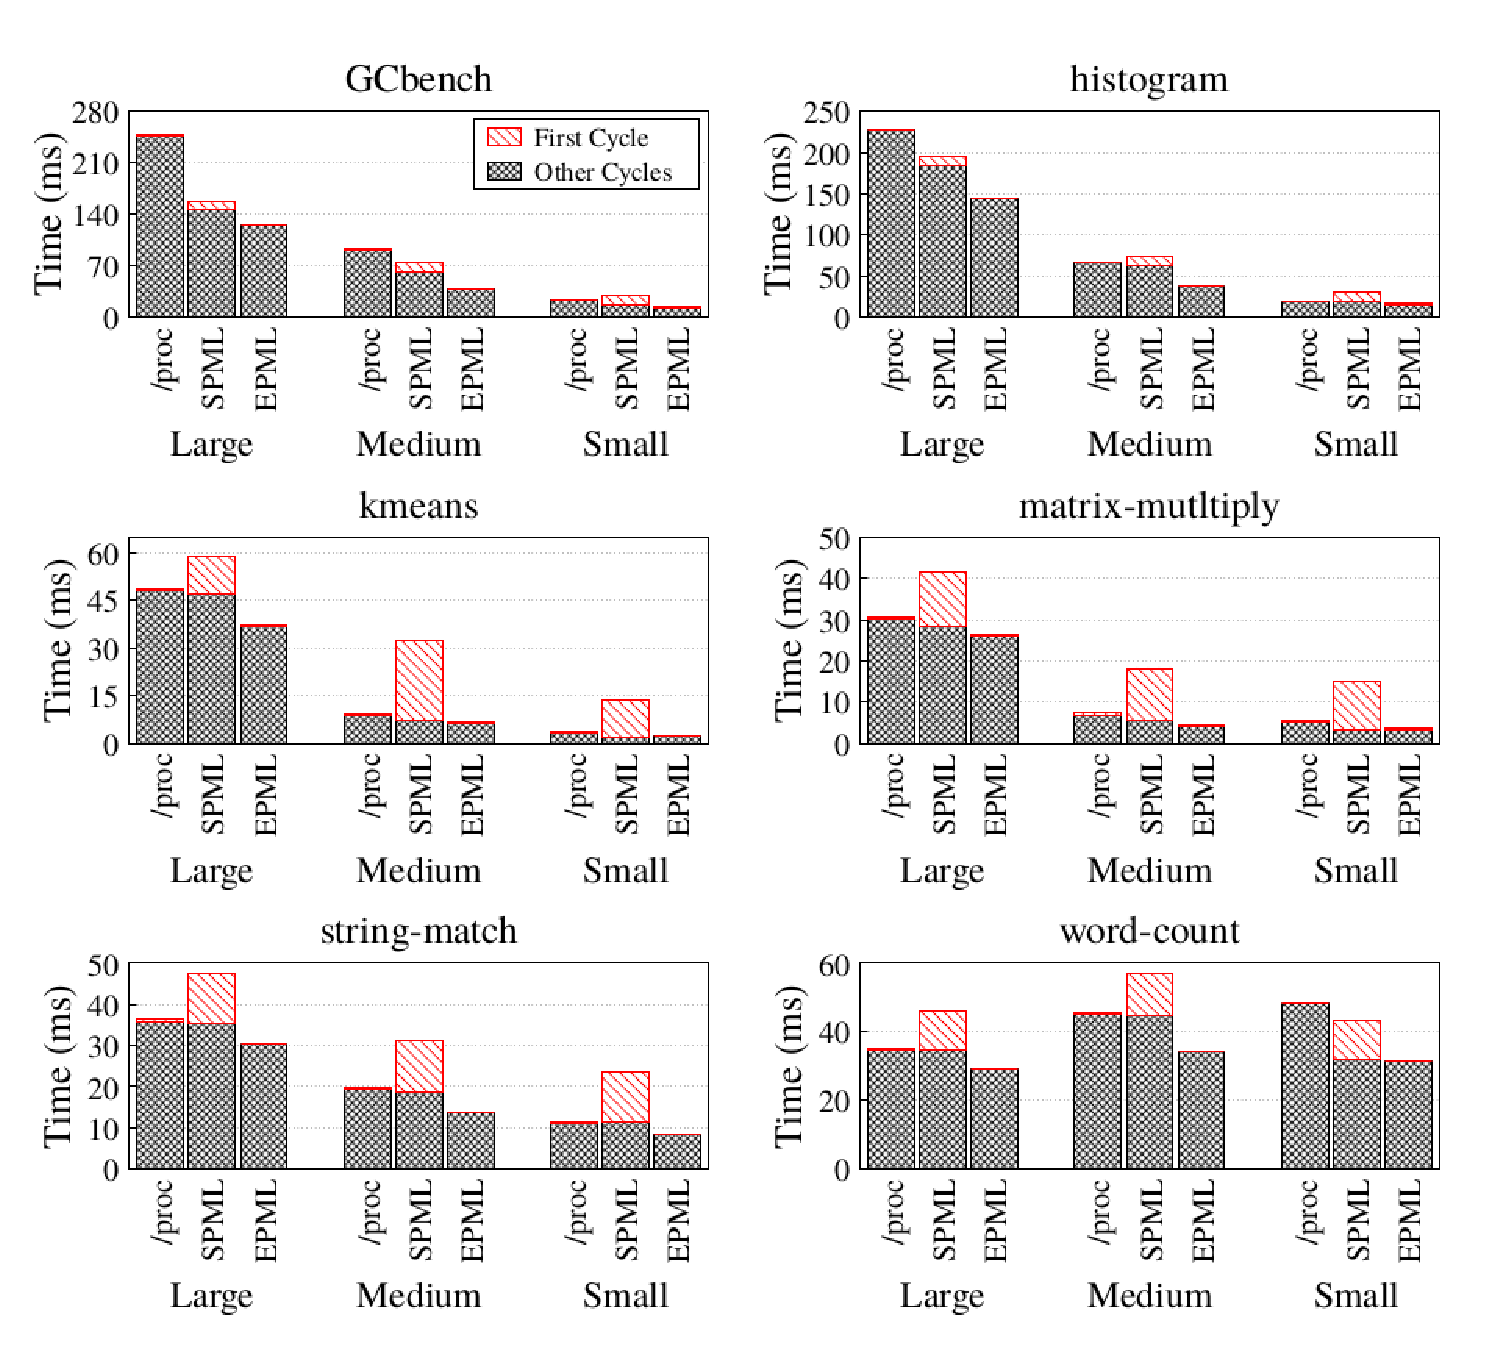
\includegraphics[width=.5\linewidth]{fig/boehm-results-tracker}		
					\caption{\scriptsize We highlight the first GC cycle during which Boehm performs reverse mapping with SPML.}
					\label{fig:boehm-results-tracker}
				\end{figure}											
			\end{block}
        \end{frame}
%%%%%%%%%%%%%%%%%%%%%%%%%%%%%%%%%%%%%%%%%%%%%%%%%%%%%%%%%%%%%%%%%%%%%%%%%%%%%%%%%%%
        \begin{frame}
			\frametitle{Evaluations Results}
			\begin{block}{Impact on applications}
				\begin{figure}[!htp]
					\centering 
					\fcolorbox{white}{white}{					
					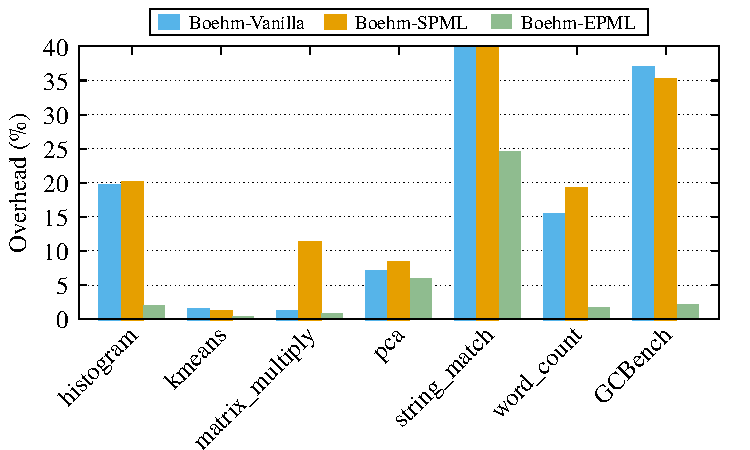
\includegraphics[width=.3\linewidth]{fig/tracked_large}
					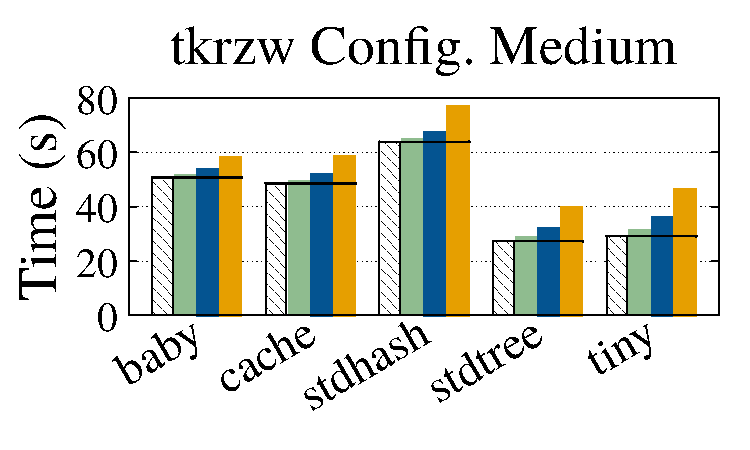
\includegraphics[width=.3\linewidth]{fig/tracked_medium}
					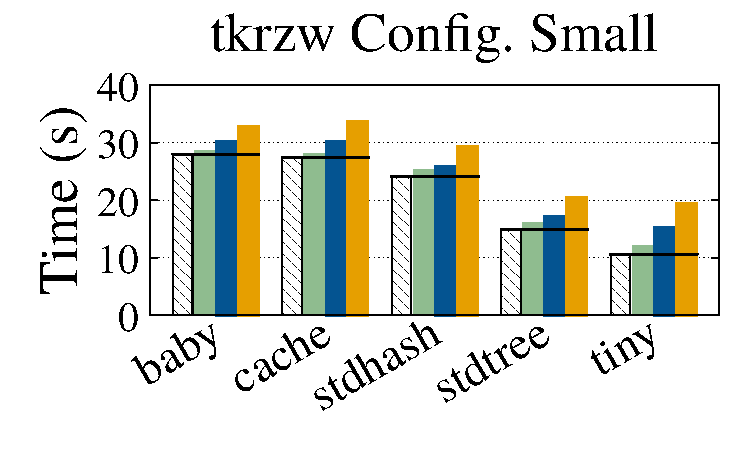
\includegraphics[width=.3\linewidth]{fig/tracked_small}
					}		
					\caption{\small Impact of Boehm GC.}
					\label{fig:boehm-results-tracked}
				\end{figure}											
			\end{block}
        \end{frame}      
%%%%%%%%%%%%%%%%%%%%%%%%%%%%%%%%%%%%%%%%%%%%%%%%%%%%%%%%%%%%%%%%%%%%%%%%%%%%%%%%%%%
        \begin{frame}
			\thispagestyle{empty}
			\frametitle{Evaluations Results}
			\begin{block}{Impact on CRIU}
				\begin{figure}[!htp]
					\centering 
					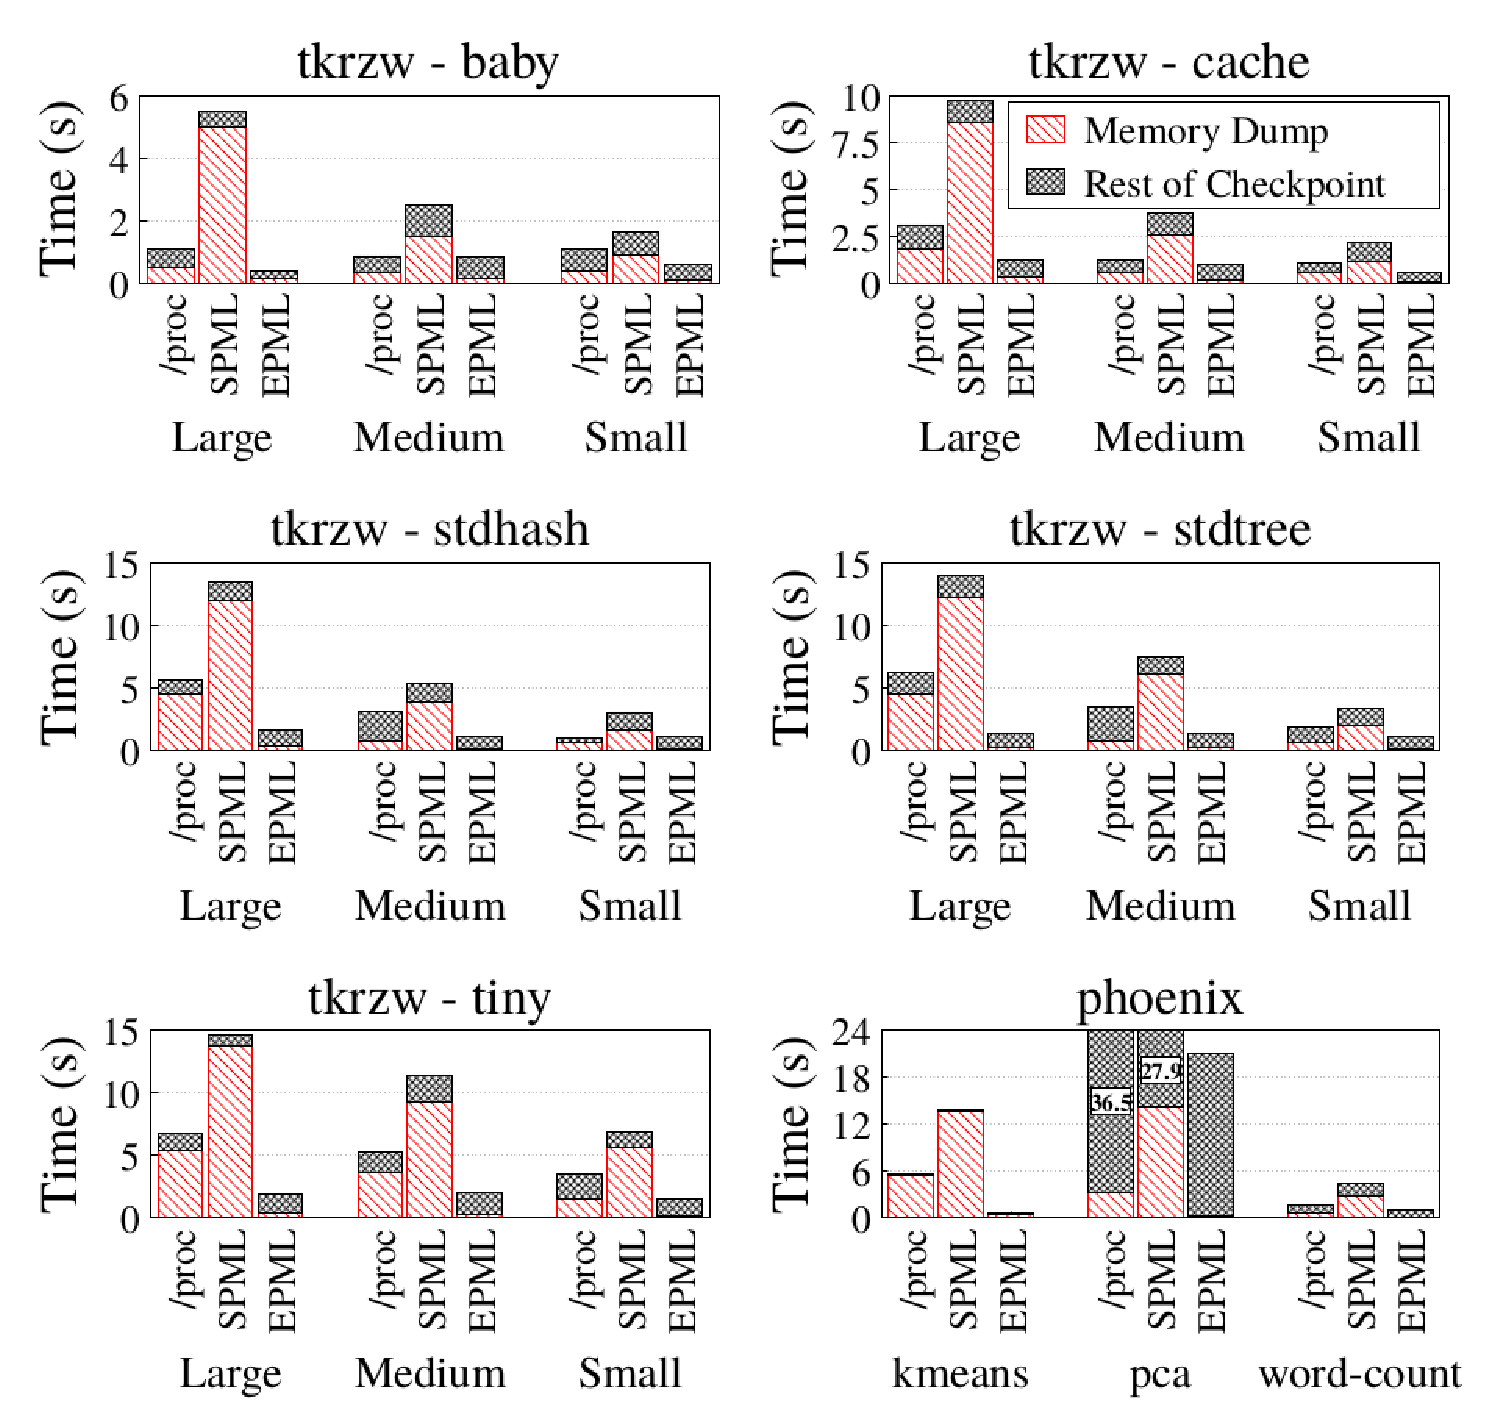
\includegraphics[width=.45\linewidth]{fig/criu-results-tracker}
					\caption{\scriptsize We highlight MD phase during which CRIU performs reverse mapping with SPML.}
					\label{fig:criu-results-tracker}
				\end{figure}											
			\end{block}
        \end{frame}        
%%%%%%%%%%%%%%%%%%%%%%%%%%%%%%%%%%%%%%%%%%%%%%%%%%%%%%%%%%%%%%%%%%%%%%%%%%%%%%%%%%%
        \begin{frame}
			\frametitle{Evaluations Results}
			\begin{block}{Impact on the checkpointed app}
				\begin{figure}[!h]
					\centering 
					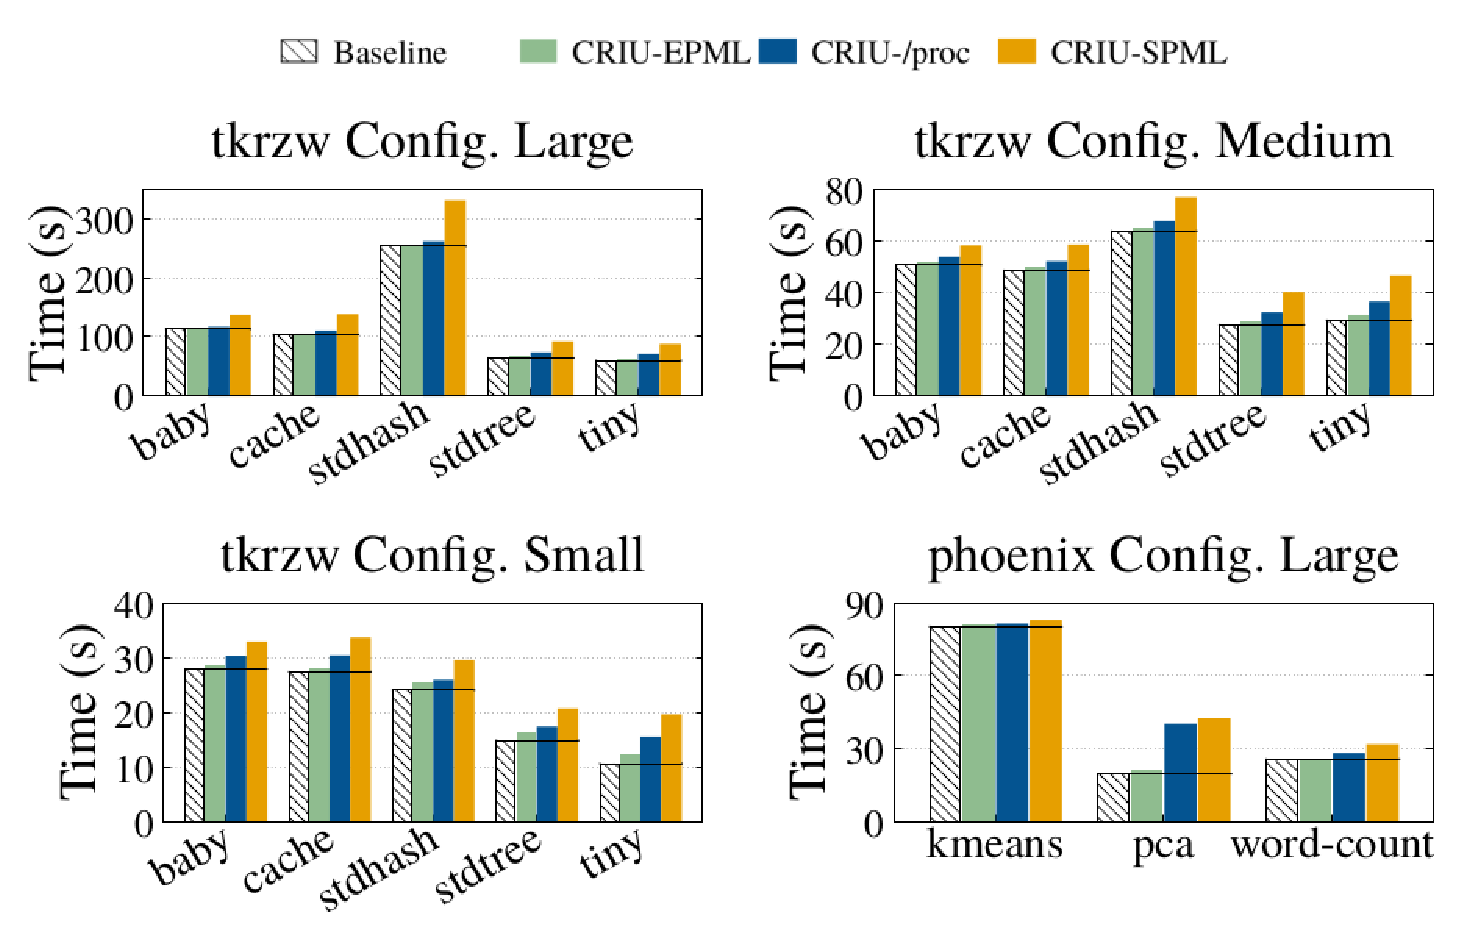
\includegraphics[width=.6\linewidth]{fig/criu-results-tracked}
				\end{figure}										
			\end{block}
        \end{frame}         
%%%%%%%%%%%%%%%%%%%%%%%%%%%%%%%%%%%%%%%%%%%%%%%%%%%%%%%%%%%%%%%%%%%%%%%%%%%%%%%%%%%
        \begin{frame}
                \frametitle{Evaluations Results}
				\begin{block}{Summary}
					\begin{itemize}
						\item Impact on the tracker
						\begin{itemize}
							\item SPML induces up to 5$\times$ slowdown on CRIU and 3$\times$ slowdown on Boehm GC.
							\item EPML brings up to 4$\times$ speedup compared to \texttt{/proc} and 13$\times$ speedup compared to SPML for CRIU; up to 2$\times$ speedup compared to \texttt{/proc} and up to 6$\times$ speedup compared to SPML.
						\end{itemize}																							
					\end{itemize}
			\end{block}
        \end{frame}  
%%%%%%%%%%%%%%%%%%%%%%%%%%%%%%%%%%%%%%%%%%%%%%%%%%%%%%%%%%%%%%%%%%%%%%%%%%%%%%%%%%%
        \begin{frame}
                \frametitle{Evaluations Results}
				\begin{block}{Summary}
					\begin{itemize}		
						\item Impact on the application performance
						\begin{itemize}
							\item \texttt{/proc}, which is the default solution implemented in both CRIU and Boehm, incurs an overhead of up to 102\% with CRIU on the Phoenix \texttt{pca} application, and up to 232\% with Boehm on the Phoenix \texttt{string-match} application.
							\item The overhead of SPML is up to 114\% with CRIU and 273\% with Boehm on the same applications.
							\item EPML leads to the lowest overhead, which is about 7\% with CRIU and 24\% with Boehm.
						\end{itemize}																							
					\end{itemize}
			\end{block}
        \end{frame}           
%%%%%%%%%%%%%%%%%%%%%%%%%%%%%%%%%%%%%%%%%%%%%%%%%%%%%%%%%%%%%%%%%%%%%%%%%%%%%%%%%%%
        \begin{frame}
		\thispagestyle{empty}
        \frametitle{Conclusion} 
			\begin{block}{Dirty Page Tracking and OoH for Intel PML}
				\begin{itemize}
					\item For wss estimation, live migration, checkpointing, GC, ...
					\item Induce high overhead on applications
				\end{itemize}
				\begin{itemize}
					\item For improving process/container checkpointing, concurrent GCs
					\item Excellent results in both reducing overhead on tracked applications and improving the tracking application
				\end{itemize}
			\end{block}
			\begin{block}{Thake Away}
				\begin{itemize}
					\item Existing sofware-based tools can be improved using hardware virtualization features
					\item When thinking hypervisor-oriented hardware virtualization features, we must think how they can also be used by processes from inside VMs, this may need few efforts
				\end{itemize}
			\end{block}							
        \end{frame}                       
%%%%%%%%%%%%%%%%%%%%%%%%%%%%%%%%%%%%%%%%%%%%%%%%%%%%%%%%%%%%%%%%%%%%%%%%%%%%%%
      
\end{document}
